\documentclass{ctexart}
\usepackage{graphicx}
\usepackage{amsmath}
\usepackage{amsthm}
\usepackage{amssymb}
\usepackage{fancyhdr}
\usepackage{ifthen}
\usepackage{syntonly}

\usepackage{listings}
\usepackage{color}


\definecolor{dkgreen}{rgb}{0,0.6,0}
\definecolor{gray}{rgb}{0.5,0.5,0.5}
\definecolor{mauve}{rgb}{0.58,0,0.82}

\lstset{ %
  language=c++,                % the language of the code
  basicstyle=\footnotesize,           % the size of the fonts that are used for the code
  backgroundcolor=\color{white},      % choose the background color. You must add \usepackage{color}
  showspaces=false,               % show spaces adding particular underscores
  showstringspaces=false,         % underline spaces within strings
  showtabs=false,                 % show tabs within strings adding particular underscores
  frame=single,                   % adds a frame around the code
  rulecolor=\color{black},        % if not set, the frame-color may be changed on line-breaks within not-black text (e.g. commens (green here))
  tabsize=4,                      % sets default tabsize to 2 spaces
  captionpos=b,                   % sets the caption-position to bottom
  breaklines=true,                % sets automatic line breaking
  breakatwhitespace=false,        % sets if automatic breaks should only happen at whitespace
  title=\lstname,                   % show the filename of files included with \lstinputlisting;
                                  % also try caption instead of title
  keywordstyle=\color{blue},          % keyword style
  commentstyle=\color{dkgreen},       % comment style
  stringstyle=\color{mauve},         % string literal style
  escapeinside={\%*}{*)},            % if you want to add LaTeX within your code
  morekeywords={*,...}               % if you want to add more keywords to the set
}
\usepackage[colorlinks, CJKbookmarks=true, linkcolor=red]{hyperref}
\pagestyle{plain}
\usepackage[raggedright]{titlesec}
\newtheorem{性质}{性质}
\newtheorem{定理}{定理}
\newtheorem{推论}{推论}
\begin{document}
\title{实验报告}
\author{计算机科学与技术系52班 杨定澄 \and 学号:2015011274 \and E-mail:892431401@qq.com}
\date{}
\maketitle
\section{作业完成情况}
使用不同算子进行求解、对象放大、双向缩放、对象移除。

对给出的六张图的缩小可见i\_reduce.jpg,i代表第i张图。

放大可见i\_enlarge.jpg,其中第六张图未进行放大。

对第三张图进行了对象移除,见test3\_remove.jpg,移除过程见视频“对象移除.mp4”

对第二张图分别用四种算子进行了求解seam图。

可见2\_seam\_1.jpg,2\_seam\_2.jpg,2\_seam\_3.jpg,2\_seam\_4.jpg
\section{使用算子}
分别使用了四种算子

\begin{lstlisting}
	for(int i=0;i<nRows;++i)
		for(int j=0;j<nCols;++j)
		{
			if(i==0||j==0||i==nRows-1||j==nCols-1)
				E[i][j]=INF;
			else
			{
				E[i][j]=0;
				for(int k=0;k<3;++k)
				{
					E[i][j]=E[i][j]+abs(mat[i][j][k]-mat[i][j+1][k])+abs(mat[i][j][k]-mat[i+1][j][k]);
					E[i][j]=E[i][j]+abs(mat[i][j][k]-mat[i][j-1][k])+abs(mat[i][j][k]-mat[i-1][j][k]);
				}
			}
		}
\end{lstlisting}
\begin{lstlisting}
	for(int i=0;i<nRows;++i)
		for(int j=0;j<nCols;++j)
		{
			if(i==0||j==0||i==nRows-1||j==nCols-1)
				E[i][j]=INF;
			else
			{
				int val=0;
				for(int k=0;k<3;++k)
				{
					val+=abs(mat[i-1][j][k]-mat[i+1][j][k]);
					val+=abs(mat[i][j-1][k]-mat[i][j+1][k]);
				}
				E[i][j]=val;
			}
		}
\end{lstlisting}
\begin{lstlisting}
	for(int i=0;i<nRows;++i)
		for(int j=0;j<nCols;++j)
		{
			if(i==0||j==0||i==nRows-1||j==nCols-1)
				E[i][j]=INF;
			else
			{
				E[i][j]=0;
				for(int k=0;k<3;++k)
				{
					int val1=mat[i-1][j+1][k]-mat[i-1][j-1][k]+2*(mat[i][j+1][k]-mat[i][j-1][k])+mat[i+1][j+1][k]-mat[i+1][j-1][k];
					int val2=mat[i-1][j-1][k]-mat[i+1][j-1][k]+2*(mat[i-1][j][k]-mat[i+1][j][k])+mat[i-1][j+1][k]-mat[i-1][j+1][k];
					E[i][j]=abs(val1)+abs(val2);
				}
			}
		}
\end{lstlisting}
\begin{lstlisting}
	for(int i=0;i<nRows;++i)
		for(int j=0;j<nCols;++j)
		{
			if(i==0||j==0||i==nRows-1||j==nCols-1)
				E[i][j]=INF;
			else
			{
				int val=0;
				for(int k=0;k<3;++k)
					val+=abs(mat[i-1][j][k]+mat[i+1][j][k]+mat[i][j+1][k]+mat[i][j-1][k]-4*mat[i][j][k]);
				E[i][j]=val;
			}
		}
\end{lstlisting}
函数SeamGraph用来求解seam图,代码如下:
\begin{lstlisting}
void SeamGraph()
{
	string name="2.png";
	Mat M=imread(name);
	int nRows=M.rows,nCols=M.cols,k=200;
	for(int i=0;i<nRows;++i)
		for(int j=0;j<nCols;++j)
			for(int k=0;k<3;++k)
				mat[i][j][k]=M.at<Vec3b>(i,j)[k];
	int delta=k;
	int nSeq=0;
	for(int T=1;T<=delta;++T)
	{
		CalcEnergyFunction(mat,nRows,nCols,E);
		for(int i=0;i<nRows;++i)
			for(int j=0;j<nCols;++j)
			{
				int e=E[i][j];
				if(i==0)
					dp1[i][j]=e;
				else
				{
					dp1[i][j]=dp1[i-1][j],from1[i][j]=j;
					if(j>0&&dp1[i][j]>dp1[i-1][j-1])
						dp1[i][j]=dp1[i-1][j-1],from1[i][j]=j-1;
					if(j+1<nCols&&dp1[i][j]>dp1[i-1][j+1])
						dp1[i][j]=dp1[i-1][j+1],from1[i][j]=j+1;
					dp1[i][j]+=e;
				}
			}
		for(int i=nRows-1,j=min_element(dp1[nRows-1],dp1[nRows-1]+nCols)-dp1[nRows-1];i>=0;--i)
		{
			++nSeq;
			seq[nSeq][3]=j;
			for(int k=0;k<3;++k)
				seq[nSeq][k]=mat[i][j][k];
			for(int k=j+1;k<nCols;++k)
				for(int l=0;l<3;++l)
					mat[i][k-1][l]=mat[i][k][l];
			j=from1[i][j];
		}
		--nCols;
	}
	for(int i=0;nSeq;i=(i+1)%nRows)
	{
		int j=seq[nSeq][3];
		for(int k=nCols;k>=j+1;--k)
		{
			for(int l=0;l<3;++l)
				mat[i][k][l]=mat[i][k-1][l];
			isDelete[i][k]=isDelete[i][k-1];
		}
		isDelete[i][j]=true;
		for(int k=0;k<3;++k)
			mat[i][j][k]=seq[nSeq][k];
		if(i==nRows-1)
			++nCols;
		nSeq--;
	}
	M=Mat(nRows,nCols,CV_8UC3);
	for(int i=0;i<nRows;++i)
		for(int j=0;j<nCols;++j)
		{
			Vec3b pixel;
			if(isDelete[i][j])
				pixel=Vec3b(255,0,0);
			else
				for(int k=0;k<3;++k)
					pixel[k]=mat[i][j][k];
			M.at<Vec3b>(i,j)=pixel;
		}
	imwrite("2_seam.png",M);
}
\end{lstlisting}

对给出的2.png分别求解seam图,效果如下

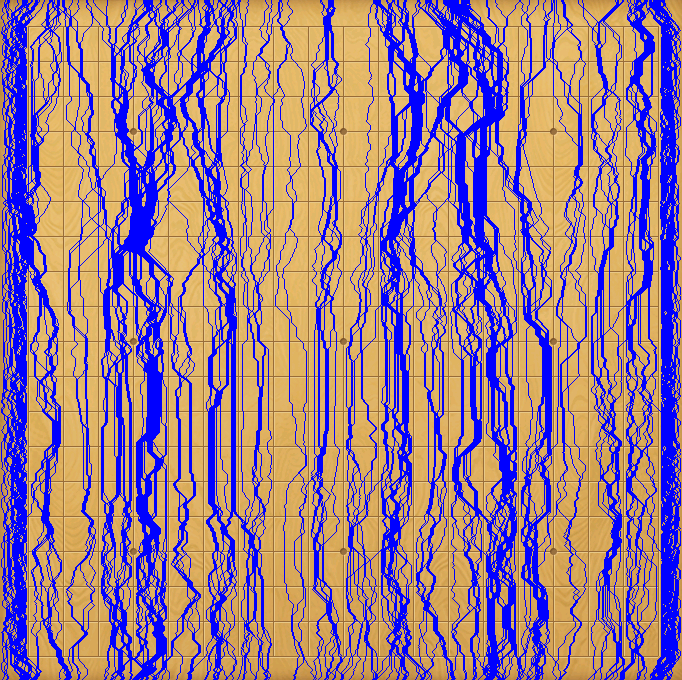
\includegraphics[width=10cm,height=10cm]{2_seam_1.png}

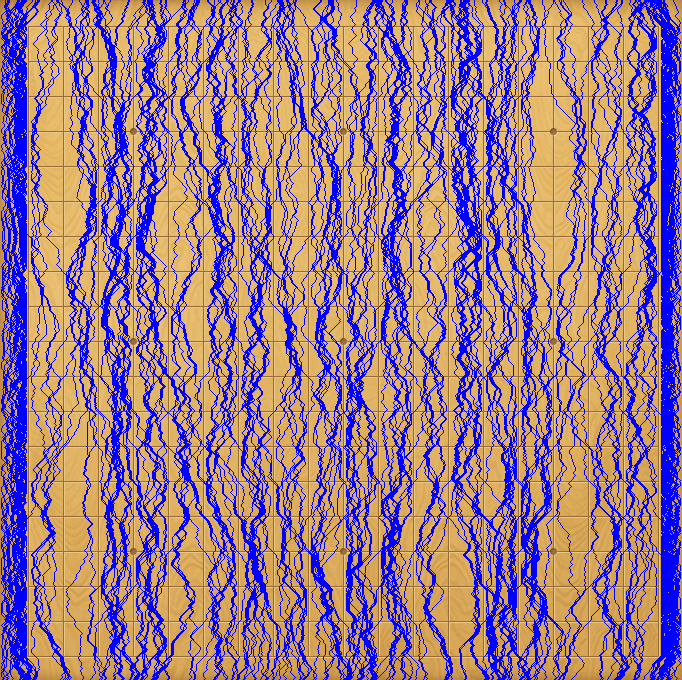
\includegraphics[width=10cm,height=10cm]{2_seam_2.png}

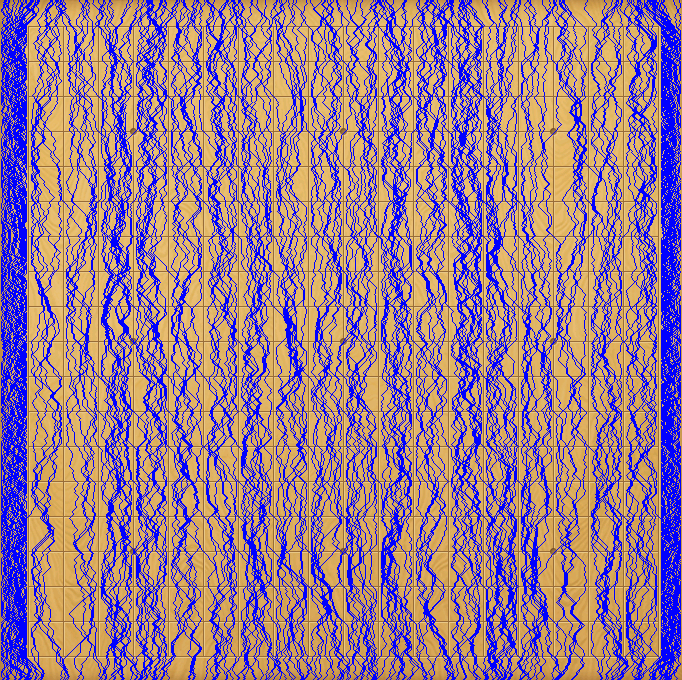
\includegraphics[width=10cm,height=10cm]{2_seam_3.png}

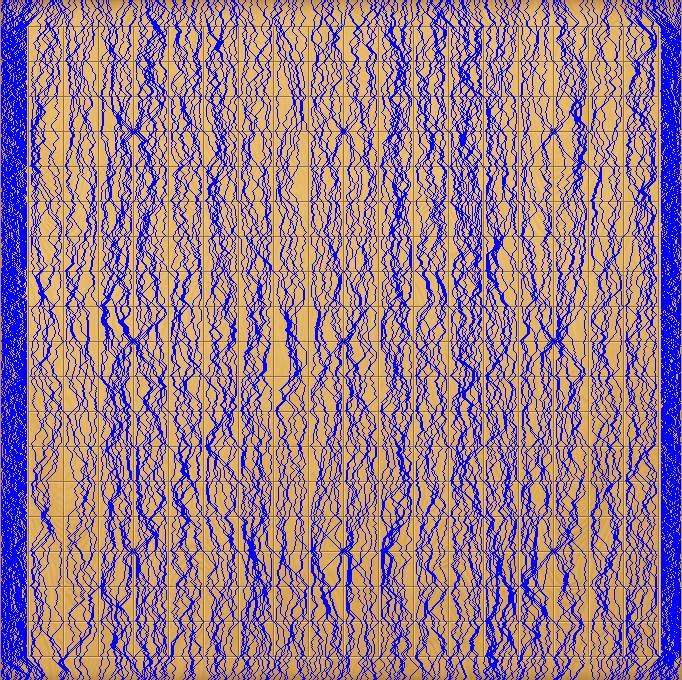
\includegraphics[width=10cm,height=10cm]{2_seam_4.png}

\section{双向缩放}
函数Reduce用来实现双向缩放。

每次分别横向、纵向求解,每次贪心选择删行还是删列,代码如下:
\begin{lstlisting}

void Reduce()
{
	string name="2.png";
	Mat M=imread(name);
	int nRows=M.rows,nCols=M.cols,goalCol=nCols/10*8,goalRow=nRows,times=nRows-goalRow+nCols-goalCol;
	for(int i=0;i<nRows;++i)
		for(int j=0;j<nCols;++j)
			for(int k=0;k<3;++k)
				mat[i][j][k]=M.at<Vec3b>(i,j)[k];
	while(nRows>goalRow||nCols>goalCol)
	{
		CalcEnergyFunction(mat,nRows,nCols,E);
		for(int i=0;i<nRows;++i)
			for(int j=0;j<nCols;++j)
			{
				int e=E[i][j];
				if(i==0)
					dp1[i][j]=e;
				else
				{
					dp1[i][j]=dp1[i-1][j],from1[i][j]=j;
					if(j>0&&dp1[i][j]>dp1[i-1][j-1])
						dp1[i][j]=dp1[i-1][j-1],from1[i][j]=j-1;
					if(j+1<nCols&&dp1[i][j]>dp1[i-1][j+1])
						dp1[i][j]=dp1[i-1][j+1],from1[i][j]=j+1;
					dp1[i][j]+=e;
				}
			}
		for(int j=0;j<nCols;++j)
			for(int i=0;i<nRows;++i)
			{
				int e=E[i][j];
				if(j==0)
					dp2[j][i]=e;
				else
				{
					dp2[j][i]=dp2[j-1][i],from2[j][i]=i;
					if(i>0&&dp2[j][i]>dp2[j-1][i-1])
						dp2[j][i]=dp2[j-1][i-1],from2[j][i]=i-1;
					if(i+1<nRows&&dp2[j][i]>dp2[j-1][i+1])
						dp2[j][i]=dp2[j-1][i+1],from2[j][i]=i+1;
					dp2[j][i]+=e;
				}
			}
		LL cost_col=*min_element(dp1[nRows-1],dp1[nRows-1]+nCols);
		LL cost_row=*min_element(dp2[nCols-1],dp2[nCols-1]+nRows);
		if(nCols>goalCol&&(nRows==goalRow||cost_col*nRows<cost_row*nCols))
		{
			for(int i=nRows-1,j=min_element(dp1[nRows-1],dp1[nRows-1]+nCols)-dp1[nRows-1];i>=0;--i)
			{
				for(int k=j+1;k<nCols;++k)
					for(int l=0;l<3;++l)
						mat[i][k-1][l]=mat[i][k][l];
				j=from1[i][j];
			}
			--nCols;
		}
		else
		{
			for(int j=nCols-1,i=min_element(dp2[nCols-1],dp2[nCols-1]+nRows)-dp2[nCols-1];j>=0;--j)
			{
				for(int k=i+1;k<nRows;++k)
					for(int l=0;l<3;++l)
						mat[k-1][j][l]=mat[k][j][l];
				i=from2[j][i];
			}
			--nRows;
		}
	}
	M=Mat(nRows,nCols,CV_8UC3);
	for(int i=0;i<nRows;++i)
		for(int j=0;j<nCols;++j)
		{
			Vec3b pixel;
			for(int k=0;k<3;++k)
				pixel[k]=mat[i][j][k];
			M.at<Vec3b>(i,j)=pixel;
		}
	imwrite("2_reduce.jpg",M);	
}
\end{lstlisting}

\section{图像放大}
函数Enlarging用来实现图像放大,假设要让列数变大k(不妨设k小于列数一半),首先删去k列,记下删去的操作,再用类似于栈的方式反向得到原图,过程中记下删除过的像素点。

接着把删除过的像素点翻倍即可,代码如下:
\begin{lstlisting}
void Enlarging()
{
	string name="test9.png";
	Mat M=imread(name);
	int goalCol=M.cols*2,nRows=M.rows,nCols=M.cols,times=abs(nCols-goalCol),k=nCols/2;
	for(int i=0;i<nRows;++i)
		for(int j=0;j<nCols;++j)
			for(int k=0;k<3;++k)
				mat[i][j][k]=M.at<Vec3b>(i,j)[k];
	while(nCols<goalCol)
	{
		int delta=min(k,goalCol-nCols);
		int nSeq=0;
		for(int T=1;T<=delta;++T)
		{
			CalcEnergyFunction(mat,nRows,nCols,E);
			for(int i=0;i<nRows;++i)
				for(int j=0;j<nCols;++j)
				{
					int e=E[i][j];
					if(i==0)
						dp1[i][j]=e;
					else
					{
						dp1[i][j]=dp1[i-1][j],from1[i][j]=j;
						if(j>0&&dp1[i][j]>dp1[i-1][j-1])
							dp1[i][j]=dp1[i-1][j-1],from1[i][j]=j-1;
						if(j+1<nCols&&dp1[i][j]>dp1[i-1][j+1])
							dp1[i][j]=dp1[i-1][j+1],from1[i][j]=j+1;
						dp1[i][j]+=e;
					}
				}
			for(int i=nRows-1,j=min_element(dp1[nRows-1],dp1[nRows-1]+nCols)-dp1[nRows-1];i>=0;--i)
			{
				++nSeq;
				seq[nSeq][3]=j;
				for(int k=0;k<3;++k)
					seq[nSeq][k]=mat[i][j][k];
				for(int k=j+1;k<nCols;++k)
					for(int l=0;l<3;++l)
						mat[i][k-1][l]=mat[i][k][l];
				j=from1[i][j];
			}
			--nCols;
		}
		for(int i=0;nSeq;i=(i+1)%nRows)
		{
			int j=seq[nSeq][3];
			for(int k=nCols;k>=j+1;--k)
			{
				for(int l=0;l<3;++l)
					mat[i][k][l]=mat[i][k-1][l];
				isDelete[i][k]=isDelete[i][k-1];
			}
			isDelete[i][j]=true;
			for(int k=0;k<3;++k)
				mat[i][j][k]=seq[nSeq][k];
			if(i==nRows-1)
				++nCols;
			nSeq--;
		}
		for(int i=0;i<=nRows;++i)
			for(int j=nCols+delta-1,k=nCols-1;k>=0;--k)
			{
				for(int l=0;l<3;++l)
					mat[i][j][l]=mat[i][k][l];
				--j;
				if(isDelete[i][k])
				{
					isDelete[i][k]=false;
					for(int l=0;l<3;++l)
						mat[i][j][l]=mat[i][k][l];
					--j;
				}
			}
		nCols+=delta;
	}
	M=Mat(nRows,nCols,CV_8UC3);
	for(int i=0;i<nRows;++i)
		for(int j=0;j<nCols;++j)
		{
			Vec3b pixel;
			for(int k=0;k<3;++k)
				pixel[k]=mat[i][j][k];
			M.at<Vec3b>(i,j)=pixel;
		}
	imwrite("test_9.png",M);
}
\end{lstlisting}
\section{对象移除}
个人认为这里主要难点在于交互,opencv的setMouseCallBack函数可以实现鼠标事件的监视。

交互的过程中,我们把原图的像素点分成三类,普通像素点是0,要删的像素点是1,要留下来的像素点是2。

我们在求解能量函数时,对于要删的,设他的能量是-INF;对于要保留的,设他的能量是INF。

接着再不断删除直到满意要删的像素点即可,代码如下:
\begin{lstlisting}
struct Marker
{
	Mat ori,img,type;
	static void on_Mouse(int event,int x,int y,int flags,void *obj)
	{
		Marker* now=static_cast<Marker*>(obj);
		if(event==CV_EVENT_LBUTTONDOWN||(event==CV_EVENT_MOUSEMOVE&&(flags&CV_EVENT_FLAG_LBUTTON)))
		{
			circle(now->img,Point(x,y),20,Scalar(0,255,0),-1);
			circle(now->type,Point(x,y),20,1,-1);
			imshow("img",now->img);
		}
		if(event==CV_EVENT_RBUTTONDOWN||(event==CV_EVENT_MOUSEMOVE&&(flags&CV_EVENT_FLAG_RBUTTON)))
		{
			circle(now->img,Point(x,y),20,Scalar(255,0,0),-1);
			circle(now->type,Point(x,y),20,2,-1);
			imshow("img",now->img);
		}
	}
	Marker(){}
	Marker(const string &name)
	{
		ori=imread(name);
		ori.copyTo(img);
		type=Mat::zeros(img.size(),CV_8UC1);
		namedWindow("img");
		setMouseCallback("img",on_Mouse,this);
		imshow("img",img);
		while(1)
		{
			int c=waitKey(0);
			if(c==27)
				break;
		}
	}
};
uchar type[maxn][maxn];
void ObjectRemove()
{
	Marker *rem=new Marker("3.jpg");
	Mat M=rem->ori,Mt=rem->type;
	int nRows=M.rows,nCols=M.cols;
	for(int i=0;i<nRows;++i)
		for(int j=0;j<nCols;++j)
		{
			for(int k=0;k<3;++k)
				mat[i][j][k]=M.at<Vec3b>(i,j)[k];
			type[i][j]=Mt.at<uchar>(i,j);
		}
	while(1)
	{
		int cntRemove=0;
		for(int i=0;i<nRows;++i)
			for(int j=0;j<nCols;++j)
				if(type[i][j]==1)
					++cntRemove;
		if(!cntRemove)
			break;
		printf("%d\n",cntRemove);
		CalcEnergyFunction(mat,nRows,nCols,E);
		for(int i=0;i<nRows;++i)
			for(int j=0;j<nCols;++j)
			{
				int e=E[i][j];
				if(type[i][j]==1)
					e=-inf;
				if(type[i][j]==2)
					e=inf;
				if(i==0)
					dp1[i][j]=e;
				else
				{
					dp1[i][j]=dp1[i-1][j],from1[i][j]=j;
					if(j>0&&dp1[i][j]>dp1[i-1][j-1])
						dp1[i][j]=dp1[i-1][j-1],from1[i][j]=j-1;
					if(j+1<nCols&&dp1[i][j]>dp1[i-1][j+1])
						dp1[i][j]=dp1[i-1][j+1],from1[i][j]=j+1;
					dp1[i][j]+=e;
				}
			}
		LL cost_col=*min_element(dp1[nRows-1],dp1[nRows-1]+nCols);
		for(int i=nRows-1,j=min_element(dp1[nRows-1],dp1[nRows-1]+nCols)-dp1[nRows-1];i>=0;--i)
		{
			for(int k=j+1;k<nCols;++k)
			{
				for(int l=0;l<3;++l)
					mat[i][k-1][l]=mat[i][k][l];
				type[i][k-1]=type[i][k];
			}
			j=from1[i][j];
		}
		--nCols;
	}
	M=Mat(nRows,nCols,CV_8UC3);
	for(int i=0;i<nRows;++i)
		for(int j=0;j<nCols;++j)
		{
			Vec3b pixel;
			for(int k=0;k<3;++k)
				pixel[k]=mat[i][j][k];
			M.at<Vec3b>(i,j)=pixel;
		}
	imwrite("test3_remove.jpg",M);	
}
\end{lstlisting}
\end{document}
